\chapter{Metodología de la Investigación}
 
\section{Diseño de la investigación}
 
En esta sección se describe el diseño, el tipo y el enfoque del trabajo de investigación, además de la población, la muestra y la operacionalización de las variables.
 
\subsection{Tipo de la investigación}
 
Se define el presente estudio como \textbf{Diseño Experimental}, dado que este enfoque busca identificar el posible efecto de una causa que es manipulada,este enfoque es principalmente utilizado por la obra \citetitle{bk_hernandez2014metodologia} creada por \cite{bk_hernandez2014metodologia}. Asimismo, en esta categoría, se categoriza como un \textbf{Diseño Experimental Puro}, debido a que se intervinieron deliberadamente una o más variables independientes —en este caso, la configuración de la arquitectura computacional, que integra un enfoque \textbf{GraphRAG Híbrido} (bases de datos vectoriales con \textit{pgvector} y de grafos con \textit{Neo4j}), la orquestación de múltiples Modelos Fundacionales como  DeepSeek y la exposición de herramientas analíticas vía el \textbf{Model Context Protocol (MCP)}— con el propósito de evaluar su impacto sobre la variable dependiente. Dicho impacto se mide a través de la precisión en la clasificación del sentimiento, la coherencia semántica en la detección de temas, y la eficiencia y relevancia en la recuperación de información del ecosistema digital electoral peruano.


\subsection{Enfoque de la investigación}
 
El estudio propuesto adopta un \textbf{enfoque cuantitativo}, esto porque de acuerdo con \cite{bk_hernandez2014metodologia} en su obra \citetitle{bk_hernandez2014metodologia}, el enfoque  propuesto se basa en la recuperación de datos para contrastar la hipótesis mediante el uso de mediciones numéricas y el uso de análisis estadístico, con el propósito de identificar patrones de conducta y validar las hipótesis presentadas previamente. Esta se evidencia en la aplicación propuesta de 10 pasos del proceso cuantitativo utilizado por el autor, la cual parte desde la formulación de la creación de la idea y concluye con la elaboración del informe de resultados. En este trabajo, indicadores como la exactitud, la coherencia temática y la latencia de procesamiento permiten evaluar de manera objetiva el desempeño del sistema de inteligencia electoral planteado.
 
\subsection{Población}
 
La población fue el conjunto de todas las publicaciones digitales en español relacionadas con el proceso electoral peruano, generadas en plataformas de redes sociales (X/Twitter), plataformas de videos cortos (TikTok), canales de contenido audiovisual (YouTube) y portales de noticias digitales durante el período de campaña presidencial analizado.
 
\subsection{Muestra}

La muestra estuvo conformada por publicaciones recolectadas de cuatro fuentes de datos independientes durante el período electoral analizado: (1) artículos y noticias digitales de los principales portales de prensa peruanos (El Comercio, La República, RPP, Diario Correo); (2) videos YouTube correspondientes a los candidatos y programas periodísticos de cobertura electoral; (3) tweets de la plataforma X/Twitter; y (4) videos y transcripciones de la red social TikTok. La extracción se delimitó mediante palabras clave electorales, \textit{hashtags} de campaña y menciones a cuentas oficiales. El criterio de delimitación temporal obedeció a la necesidad de capturar el período de mayor actividad del ecosistema digital electoral, excluyendo etapas de baja intensidad que distorsionarían los patrones de sentimiento y emergencia de temas.

\textbf{Tamaño muestral y técnica de muestreo.} En la corrida completa del pipeline se procesaron \textbf{40\,974 documentos}, recolectados a lo largo de \textbf{96 días consecutivos} (del 1 de enero al 6 de abril de 2026), tras la aplicación de los filtros pre-LLM de la arquitectura Medallion. Dado que el universo de publicaciones digitales es dinámico, continuo y no tiene un marco muestral cerrado ni un tamaño poblacional finito y conocido, se adoptó un \textbf{muestreo no probabilístico por conveniencia} \parencite{bk_hernandez2014metodologia}: la muestra quedó definida por los documentos accesibles a través de los scrapers y las APIs disponibles en el período delimitado, filtrados por los criterios de relevancia electoral descritos.

\textbf{Criterios de inclusión}: (a) publicación en español; (b) fecha de publicación dentro del período de campaña presidencial analizado; (c) contenido textual que mencione al menos un candidato presidencial o un término del diccionario electoral; (d) fuente perteneciente a los cuatro canales definidos (noticias digitales, X/Twitter, YouTube, TikTok).

\textbf{Criterios de exclusión}: (a) publicaciones duplicadas o reediciones sin contenido nuevo; (b) documentos con menos de 30 tokens útiles tras el preprocesamiento; (c) contenido en idioma distinto al español; (d) publicaciones fuera del período temporal delimitado.

\textbf{Representatividad.} Dada la técnica de muestreo no probabilístico utilizada, la muestra \textbf{no es estadísticamente representativa} del universo completo de publicaciones digitales sobre las elecciones peruanas 2026. Los resultados tienen validez interna para los canales, medios y período analizados, pero no permiten generalizar estadísticamente al conjunto de toda la conversación digital electoral. Esta limitación se reconoce explícitamente y deberá considerarse al interpretar los indicadores producidos por el sistema.

\subsection{Operacionalización de variables}
 
En la Tabla \ref{4:table1} se muestra la operación de las variables correspondientes al estudio propuesto.
\begingroup
\begin{longtable}{M{3cm}M{4.2cm}M{3.6cm}M{4.8cm}}
    \caption[Matriz de operacionalización de variables]{Matriz de operacionalización de variables.}
    \label{4:table1}
    \centering
    \small
    \tabularnewline \specialrule{.1em}{.05em}{.05em}
    VARIABLE & DIMENSIÓN & INDICADOR & CÁLCULO \\
    \specialrule{.1em}{.05em}{.05em}

    % Variable independiente
    \multirow{10}{3cm}[-6ex]{\centering Independiente: Arquitectura de recuperacion (MCP vs RAG)}
    & \multirow{5}{4.2cm}[-1ex]{\centering Arquitectura de Extracción y Análisis (LLMs)}
    & \multicolumn{2}{c}{\centering Configuración del pipeline de análisis} \\
    \cline{3-4}
    & & \multirow{4}{3.6cm}[0ex]{\centering Efectividad del análisis predictivo}
    & Exactitud en clasificación de sentimiento y detección de actores \\
    \cline{4-4}
    & & & Corrección de respuesta (Answer Correctness) (C\textsubscript{v}) \\
    \cline{4-4}
    & & & Latencia de procesamiento e ingesta (ms) \\
    \cline{2-4}
    & \multirow{5}{4.2cm}[-1ex]{\centering Arquitectura de Recuperación (Grafos y Vectores)}
    & \multicolumn{2}{c}{\centering Configuración Neo4j y pgvector + MCP Server} \\
    \cline{3-4}
    & & \multirow{4}{3.6cm}[0ex]{\centering Efectividad de recuperación (Retrieval)}
    & Latencia de consulta vía Model Context Protocol (ms) \\
    \cline{4-4}
    & & & Exactitud en selección de herramientas (Tool Selection Accuracy) \\

    \hline

% Variable dependiente
\multirow{13}{=}{Dependiente: Calidad/eficacia del sistema de análisis}
& \multirow{4}{=}{Sentimiento ciudadano}
& \multirow{2}{=}{Polaridad de sentimiento}
& Positivo: $S(d,e) > 0$ \\* \cline{4-4}
& & & Negativo: $S(d,e) < 0$ \\* \cline{3-4}
& & Intensidad del sentimiento & Score continuo $[-1, 1]$ \\* \cline{2-4}
& \multirow{6}{=}{Conversación digital electoral}
& \multirow{2}{=}{Metainformación del corpus}
& Volumen de publicaciones por período \\* \cline{4-4}
& & & Distribución por fuente de datos \\* \cline{3-4}
& & Temas relevantes & Número y coherencia de temas detectados \\* \cline{3-4}
& & \multirow{2}{=}{Evolución temporal}
& Velocidad de emergencia de temas \\* \cline{4-4}
& & & Cambios de sentimiento por evento electoral \\* \cline{2-4}
& \multirow{3}{=}{Polarización de la percepción mediática digital}
& ISN por fuente
& $ISN_f(e,t)$ (insumo) \\* \cline{3-4}
& & ICMC (magnitud) & Desviación estándar del ISN entre fuentes; umbral $>25$ \\* \cline{3-4}
& & IDN (estructura) & $|ISN_{f_1}-ISN_{f_2}|$ por par; umbral $>50$ \\
\specialrule{.1em}{.05em}{.05em}
\end{longtable}
\endgroup
\begin{flushleft}
    \small Fuente: Elaboración propia.
\end{flushleft}
 
El presente estudio busca abordar la problemática del análisis de la percepción actual proyectada por parte de los distintos canales de comunicación en ecosistemas digitales de carácter electoral, implementando un pipeline automatizado de inteligencia electoral que integra análisis de sentimientos con LLMs y detección dinámica de temas mediante un enfoque híbrido LLM con catálogo incremental sobre un corpus multicanal de publicaciones en español.

La variable dependiente —la percepción actual proyectada por los canales de comunicación en ecosistemas digitales— se operacionaliza a través del
sentimiento expresado en publicaciones digitales hacia cada candidato presidencial,
desagregado por fuente de información, período temporal y tema relevante asociado.
Siguiendo la metodología GraphRAG descrita en la arquitectura del sistema, un mismo
segmento de texto puede expresar sentimientos distintos hacia distintos candidatos, lo que
permite capturar la complejidad real del discurso político ciudadano a nivel de aspecto
(\textit{Aspect-Based Sentiment Analysis}).
 
\section{Técnicas de recolección de datos}
 
La información recopilada para el estudio propuesto están conformado por variables de carácter cuantitativo —como el volumen de publicaciones por período y el \textit{score} continuo de sentimiento $[-1, 1]$— y variables cualitativas —como el texto de las publicaciones, las transcripciones de videos, los fragmentos clave que justifican el sentimiento y las entidades extraídas por el LLM—. Para obtener el corpus multicanal, se diseñaron e implementaron cuatro módulos extractores independientes dentro del componente de recolección (\texttt{scrap-information}), abarcando: (1) portales de noticias digitales, (2) la plataforma X/Twitter, (3) la red de videos YouTube y (4) la red social de videos cortos TikTok. El flujo de estas operaciones de extracción alimenta la capa de datos crudos (\textit{Raw}) de la arquitectura del sistema, tal como se ilustra en el esquema general de la Figura \ref{4:fig1}.
 
\begin{figure}[!ht]
    \begin{center}
        \resizebox{0.95\textwidth}{!}{\input{3/figures/flujo_recoleccion.tex}}
        \caption[Flujograma de recolección de los conjuntos de datos del corpus electoral]{Flujograma de recuperación de la información del corpus electoral: noticias digitales, transcripciones de videos de YouTube y tweets de X/Twitter, con sus respectivos procesos de filtrado y almacenamiento en la capa Bronze de la arquitectura Medallion.\\
            Fuente: Elaboración propia.}
        \label{4:fig1}
    \end{center}
\end{figure}
 
De manera específica, las técnicas computacionales empleadas para la recolección multicanal se dividen en los siguientes módulos operacionales:
\begin{itemize}
    \item \textbf{Módulo de Noticias (\textit{Web Scraping}):} Utiliza \textit{scripts} automatizados en Python diseñados específicamente para analizar la estructura de los principales diarios nacionales (El Comercio, La República, RPP, Diario Correo), extrayendo el titular, el cuerpo de la noticia, la fecha de publicación y la URL de origen.
    \item \textbf{Módulo de X/Twitter (\textit{API Integration}):} Emplea adaptadores de conexión (como \texttt{twitterapi\_io}) para capturar \textit{tweets}, respuestas e hilos relevantes mediante la inyección de parámetros de búsqueda específicos, gestionando la paginación y los límites de peticiones (\textit{rate limits}).
    \item \textbf{Módulo de YouTube (\textit{API \& Scraping}):} Encargado de la extracción de metadatos de videos electorales y de la transcripción de su contenido audiovisual, capturando el discurso de candidatos, periodistas y comunicadores políticos en programas y entrevistas difundidos en la plataforma.
    \item \textbf{Módulo de TikTok (\textit{Scraping especializado}):} Desarrollado para capturar la conversación en formatos de video corto, extrayendo las descripciones de las publicaciones (\textit{captions}), etiquetas temáticas (\textit{hashtags}) y métricas de viralidad.
\end{itemize}

Asimismo, para identificar y filtrar las publicaciones relevantes para el análisis, se
definió un diccionario de palabras clave y aliases electorales que incluye los nombres
completos, apodos, partidos y hashtags de los candidatos presidenciales en liza, así como
términos relacionados con los principales temas de la campaña: economía, seguridad,
educación, salud, corrupción y gobernabilidad.
 
%%%%%%%%%%%%%%%%%%%%%%%%%%%%%%%%%%%%%%%%%%%%%%%%%%%%%%%%%%%%%%%%%%%%%%%%%%%%%%%%
%%%%%%%%%%%%%%%%%%%%%%%%%%%%%%%%%%%%%%%%%%%%%%%%%%%%%%%%%%%%%%%%%%%%%%%%%%%%%%%%
%%%%%%%%%%%%%%%%%%%%%%%%%%%%%%%%%%%%%%%%%%%%%%%%%%%%%%%%%%%%%%%%%%%%%%%%%%%%%%%%

\section{Técnicas para el procesamiento y análisis de la información}
 
\subsection{Metodología de implementación de la solución}
 
Según lo explicado en el Capítulo II del presente trabajo, internamente en los sistemas de
analítica de negocio, la Minería de Datos y Big Data, las tres principales metodologías más usadas son
SEMMA, CRISP-DM y KDD \parencite{tec_moine2011metodologiasdm}. Para elegir la
metodología de implementación, se creó la Tabla \ref{4:table2} con el propósito de  realizar una comparativa de las variables empleadas por los distintos antecedentes presentados para el estudio propuesto.
 
\vspace{2ex}
\begingroup
\renewcommand\arraystretch{1.2}
\small
\begin{longtable}{p{3cm}p{2.5cm}p{2.5cm}p{6cm}}
\caption[Cuadro comparativo para la selección de la metodología]{Cuadro comparativo para la selección de la metodología de implementación.}
\label{4:table2} \\
\specialrule{.1em}{.05em}{.05em}
\centering\textbf{Metodología} & \centering\textbf{Cantidad de referencias} & \centering\textbf{Número de pasos} & \centering\arraybackslash\textbf{Nombre de los pasos} \\
\specialrule{.1em}{.05em}{.05em}
\endfirsthead

% Este bloque se repetirá automáticamente si la tabla salta a la siguiente página
\caption[]{Cuadro comparativo para la selección de la metodología (continuación).} \\
\specialrule{.1em}{.05em}{.05em}
\centering\textbf{Metodología} & \centering\textbf{Cantidad de referencias} & \centering\textbf{Número de pasos} & \centering\arraybackslash\textbf{Nombre de los pasos} \\
\specialrule{.1em}{.05em}{.05em}
\endhead

CRISP-DM
& 2
& 6
& \begin{itemize}[label={--},nosep,leftmargin=*]
\item Comprensión de la idea de negocio.
\item Análisis de la información recuperada.
\item Procesamiento de la información.
\item Construcción del modelo.
\item Validación.
\item Implementación.
\end{itemize} \\ 
\hline
Grupo A
& 2
& 6
& \begin{itemize}[label={--},nosep,leftmargin=*]
\item Planteamiento de la problemática encontrada.
\item Obtención la información multicanal.
\item Preprocesamiento de texto.
\item Análisis con LLM.
\item Validación de resultados.
\item Despliegue.
\end{itemize} \\ 
\hline
Grupo B
& 2
& 5
& \begin{itemize}[label={--},nosep,leftmargin=*]
\item Obtención de datos.
\item Preprocesamiento y filtrado.
\item Análisis de sentimientos.
\item Detección de temas.
\item Evaluación.
\end{itemize} \\ 
\hline
Grupo C
& 2
& 5
& \begin{itemize}[label={--},nosep,leftmargin=*]
\item Planteamiento de la problemática encontrada.
\item Obtención de la información.
\item Preprocesamiento de la información recuperada.
\item Creación del modelo y análisis.
\item Evaluación.
\end{itemize} \\ 
\hline
Grupo D
& 1
& 4
& \begin{itemize}[label={--},nosep,leftmargin=*]
\item Obtención de datos.
\item Preprocesamiento.
\item Análisis LLM y clustering.
\item Evaluación.
\end{itemize} \\ 
\specialrule{.1em}{.05em}{.05em}
\end{longtable}
\endgroup
\begin{flushleft}
    \small Fuente: Elaboración propia.
\end{flushleft}
 
De las tres metodologías señaladas por \citeauthor{tec_moine2011metodologiasdm}, la mayor parte de los antecedentes analizados siguen secuencias de actividades enmarcadas en CRISP-DM, abarcando etapas como en entendimiento del negocio, la recuperación de la información y el procesamiento los datos, la creación del modelo y la evaluación de los resultados. Asimismo, las siguientes características identificadas en los antecedentes influyeron en la selección de la metodología CRISP-DM para el presente estudio:

 
\begin{itemize}
    \item La metodología contempla entre sus fases la comprensión del negocio además
    de la parte técnica. Esta fase es crucial ya que en ella se define el problema a resolver
    —la falta de un sistema de análisis automatizado de percepción pública electoral en
    —la falta de un sistema de análisis automatizado de percepción pública electoral con procesamiento por lotes diario (near-real-time)— y se establecen los objetivos del sistema.
 
    \item Ayuda a los responsables del proyecto en la planificación y toma de decisiones
    (fase de Despliegue) a partir de los resultados obtenidos, convirtiendo los indicadores
    del sistema en oportunidades para mejorar la campaña de inteligencia electoral.
 
    \item Permite evaluar de manera continua los datos y las configuraciones del modelo a lo largo de todo el proceso, con el objetivo de construir el pipeline más adecuado. Estas evaluaciones resultan clave para interpretar los resultados y tomar decisiones sobre la arquitectura del sistema.

\item A diferencia de SEMMA, que inicia directamente con el muestreo sin enfatizar la comprensión del contexto, y de KDD, cuyo enfoque es más técnico y centrado en métricas sin considerar el entorno del negocio, CRISP-DM incorpora de forma explícita la formulación del problema, aspecto presente en el desarrollo de este trabajo.

\end{itemize}
 
Todas las etapas de la metodología que hemos escogido, adaptada al contexto de la
inteligencia electoral con LLMs, lo describimos en la Figura \ref{4:fig2}.
 
\begin{figure}[!ht]
    \begin{center}
        \includegraphics[width=1\textwidth]{3/figures/metodologia_crispdm.png}
        \caption[Metodología CRISP-DM adaptada al sistema de inteligencia electoral con LLMs]{Metodología CRISP-DM adaptada al sistema de inteligencia electoral con LLMs, mostrando las seis fases, su carácter iterativo y los entregables de cada etapa.\\
            Fuente: Elaboración propia.}
        \label{4:fig2}
    \end{center}
\end{figure}
 
Durante la ejecución de la metodología, se definió construir un pipeline
de análisis multicanal que integra análisis de sentimientos con LLMs, detección dinámica
de temas mediante un enfoque híbrido LLM con catálogo incremental y un grafo de conocimiento con Neo4j, arquitectura denominada
\textbf{Pipeline de Inteligencia Electoral Basado en LLMs y Grafo de Conocimiento}. De acuerdo a la literatura de los antecedentes revisados,
se analizaron las siguientes posibles fuentes de datos a incorporar:
 
\begin{itemize}
    \item \textbf{Noticias digitales}: \cite{pr_alvarez2023llm_political}, \cite{pr_mendonca2025bertopic_political}, \cite{pr_alvi2023twitter_election_review}.
    \item \textbf{Publicaciones en X/Twitter}: \cite{pr_gujral2024llm_elections}, \cite{pr_alvi2023twitter_election_review}, \cite{pr_mendonca2025bertopic_political}.
    \item \textbf{Comentarios de YouTube}: \cite{pr_chen2024combating_misinformation}.
    \item \textbf{Datos de encuestas electorales}: \cite{pr_gujral2024llm_elections}.
\end{itemize}
 
De las anteriores fuentes, los datos de encuestas electorales no fueron incluidos en el
pipeline principal de procesamiento ya que se utilizan exclusivamente como conjunto de
validación para calibrar los indicadores del sistema, y no como información entrante para el
análisis de sentimientos. Finalmente, fueron seleccionadas las cuatro fuentes principales
—noticias digitales, X/Twitter, transcripciones de videos de YouTube y posts de TikTok—
cuya arquitectura de recolección, procesamiento y análisis se detalla en las subsecciones
siguientes.
 
El marco de trabajo del sistema propuesto, denominado \textbf{Pipeline GraphRAG
Electoral}, se estructura según la arquitectura Medallion en tres capas de datos
(Bronze, Silver y Gold) y cinco etapas de procesamiento, como vemos en la
Figura \ref{4:fig3}.
 
\begin{figure}[!ht]
    \begin{center}
        \includegraphics[width=0.92\textwidth]{3/figures/framework_graphrag.png}
        \caption[Marco de trabajo del Pipeline GraphRAG Electoral propuesto]{Marco de trabajo del Pipeline GraphRAG Electoral: arquitectura Medallion con tres capas de datos (Bronze, Silver, Gold) y cinco etapas de procesamiento desde la ingesta hasta la generación de indicadores de percepción pública.\\
            Fuente: Elaboración propia.}
        \label{4:fig3}
    \end{center}
\end{figure}
 
\subsubsection{Entendimiento del negocio}
 
En la fase inicial, se definió el problema a partir de la comprensión del contexto del proceso electoral peruano y la necesidad de contar con un sistema automatizado de inteligencia electoral. Las actividades y tareas correspondientes a esta etapa se detallan en la Tabla \ref{4:table3}.

 
\vspace{2ex}
\begingroup
\renewcommand\arraystretch{1.2} 
\small 
\begin{longtable}{p{5cm}p{5cm}p{5cm}} 
\caption[Plan de Ejecución de la fase Entendimiento del negocio]{Plan de Ejecución de la fase Entendimiento del negocio.}
\label{4:table3} \\ 
\specialrule{.1em}{.05em}{.05em}
\centering\textbf{Plan de Ejecución} & \centering\textbf{Alcance} & \centering\arraybackslash\textbf{Acciones} \\
\specialrule{.1em}{.05em}{.05em}
\endfirsthead

% Esto aparecerá automáticamente si la tabla salta a una nueva página
\caption[]{Plan de Ejecución de la fase Entendimiento del negocio (continuación).} \\
\specialrule{.1em}{.05em}{.05em}
\centering\textbf{Plan de Ejecución} & \centering\textbf{Alcance} & \centering\arraybackslash\textbf{Acciones} \\
\specialrule{.1em}{.05em}{.05em}
\endhead

Plantear el problema, los objetivos y las hipótesis.
& Planteamiento del problema principal, así como de los objetivos generales y específicos y las hipótesis de investigación.
& \begin{itemize}[label={--},nosep,leftmargin=*]
\item Identificar la brecha existente en el análisis de la percepción electoral digital.
\item Establecer los objetivos del sistema de inteligencia electoral.
\item Formular las hipótesis del estudio.
\end{itemize} \\ 
\hline
Desarrollar el marco teórico de la investigación.
& Revisión de estudios previos relacionados con el análisis de sentimientos en contextos políticos, LLMs y detección de temas.
& \begin{itemize}[label={--},nosep,leftmargin=*]
\item Buscar literatura académica sobre el uso de LLMs en escenarios electorales.
\item Revisar material sobre BERTopic y GraphRAG aplicado a datos políticos.
\end{itemize} \\ 
\hline
Definir la metodología y la arquitectura del sistema.
& Selección de la metodología de trabajo y diseño de la arquitectura del pipeline.
& \begin{itemize}[label={--},nosep,leftmargin=*]
\item Analizar metodologías propuestas en la literatura.
\item Escoger la metodología CRISP-DM.
\item Diseñar la arquitectura tipo Medallion del sistema.
\end{itemize} \\ 
\specialrule{.1em}{.05em}{.05em}
\end{longtable}
\endgroup
\begin{flushleft}
\small Fuente: Elaboración propia.
\end{flushleft}
 
\textbf{Actividad 1: Plantear el problema, los objetivos e hipótesis}
 
Aquí vemos la manera en que identificamos la brecha existente en el análisis automatizado de la percepción pública electoral digital en el Perú, se expresan los objetivos de la investigación a la par que se plantean las hipótesis que guiarán el trabajo experimental.
 
\textbf{Entregable}: Problema, objetivos e hipótesis definidos.
 
\textbf{Actividad 2: Desarrollar el marco teórico de la investigación}
 
Ya con los objetivos definidos, realizamos la investigación de antecedentes académicos relacionados con el uso de LLMs en contextos electorales, minería de sentimientos político en español, detección dinámica de temas y sistemas GraphRAG. Se elaboró el marco teórico y conceptual descritos en el Capítulo II del presente trabajo.
 
\textbf{Entregable}: Marco teórico, antecedentes y conceptos operacionales de la investigación.
 
\textbf{Actividad 3: Definir metodología y arquitectura del sistema}
 
Luego de revisar los antecedentes y comparar las metodologías utilizadas por cada autor, se seleccionó CRISP-DM como metodología de implementación y se diseñó la arquitectura Medallion del pipeline GraphRAG Electoral.
 
\textbf{Entregable}: Metodología de implementación y arquitectura del sistema.
 
\subsubsection{Análisis de los datos}
 
Durante la segunda fase se llevaron a cabo la recolección de datos y el análisis estadístico exploratorio del corpus electoral multicanal. La información empleada incluye publicaciones provenientes de las cuatro fuentes principales (noticias digitales, X/Twitter, YouTube y TikTok), recopiladas durante el período de campaña presidencial. Las actividades y las tareas correspondientes se detallan en la Tabla \ref{4:table4}.
 
\vspace{2ex}
\begingroup
\renewcommand\arraystretch{1.2}
\small
\begin{longtable}{p{4cm}p{5.5cm}p{5.5cm}}
\caption[Plan de Ejecución de la fase Análisis de los datos]{Plan de Ejecución de la fase Análisis de los datos.}
\label{4:table4} \\
\specialrule{.1em}{.05em}{.05em}
\centering\textbf{Plan de Ejecución} & \centering\textbf{Alcance} & \centering\arraybackslash\textbf{Acciones} \\
\specialrule{.1em}{.05em}{.05em}
\endfirsthead

% Este bloque se repetirá automáticamente si la tabla salta a la siguiente página
\caption[]{Plan de Ejecución de la fase Análisis de los datos (continuación).} \\
\specialrule{.1em}{.05em}{.05em}
\centering\textbf{Plan de Ejecución} & \centering\textbf{Alcance} & \centering\arraybackslash\textbf{Acciones} \\
\specialrule{.1em}{.05em}{.05em}
\endhead

Construir corpus de noticias digitales.
& Construcción del corpus de artículos y titulares de los principales portales de prensa peruanos (capa Bronze).
& \begin{itemize}[label={--},nosep,leftmargin=*]
\item Diseñar scrapers para portales de noticias objetivo.
\item Recolectar artículos con URL, fecha, titular y texto.
\item Almacenar datos crudos en capa Bronze.
\end{itemize} \\ 
\hline
Construir corpus de X/Twitter.
& Construcción del corpus de tweets relacionados con los candidatos presidenciales mediante la API de X.
& \begin{itemize}[label={--},nosep,leftmargin=*]
\item Configurar conexión con la API Filtered Stream de X.
\item Definir palabras clave, hashtags y cuentas de interés.
\item Almacenar tweets con metadatos en capa Bronze.
\end{itemize} \\ 
\hline
Construir corpus de YouTube.
& Construcción del corpus de transcripciones de videos electorales de YouTube.
& \begin{itemize}[label={--},nosep,leftmargin=*]
\item Identificar videos electorales mediante búsqueda y canales de interés.
\item Extraer transcripción y metadatos del video con \texttt{yt-dlp}.
\item Almacenar transcripciones crudas en capa Bronze.
\end{itemize} \\
\hline
Construir corpus de TikTok.
& Construcción del corpus de posts electorales de TikTok mediante scraper independiente.
& \begin{itemize}[label={--},nosep,leftmargin=*]
\item Identificar cuentas y rangos de fechas objetivo de cobertura electoral.
\item Recolectar posts con descripción, hashtags y metadatos vía Playwright.
\item Almacenar posts crudos en capa Bronze.
\end{itemize} \\
\hline
Realizar análisis exploratorio del corpus.
& Análisis estadístico y exploratorio de las variables del corpus para cada fuente de datos.
& \begin{itemize}[label={--},nosep,leftmargin=*]
\item Describir distribución temporal y por fuente.
\item Analizar longitud de textos y vocabulario.
\item Identificar candidatos más mencionados.
\end{itemize} \\ 
\specialrule{.1em}{.05em}{.05em}
\end{longtable}
\endgroup
\begin{flushleft}
    \small Fuente: Elaboración propia.
\end{flushleft}
 
\textbf{Actividad 1: Construir corpus de noticias digitales}
 
De acuerdo a la Figura \ref{4:fig1}, en esta actividad se construyó el corpus de artículos de noticias digitales mediante scrapers diseñados en Python para los portales de prensa peruanos seleccionados. El proceso de recolección siguió el flujo de la Figura \ref{4:fig4}.
 
\begin{figure}[!ht]
    \begin{center}
        \resizebox{0.85\textwidth}{!}{\input{3/figures/flujo_scraping_noticias.tex}}
        \caption[Proceso de recolección del corpus de noticias digitales]{Proceso de recolección del corpus de noticias digitales: desde la identificación de portales objetivo hasta el almacenamiento en la capa Bronze de la arquitectura Medallion.\\
            Fuente: Elaboración propia.}
        \label{4:fig4}
    \end{center}
\end{figure}
 
\textbf{Entregable}: Corpus de noticias digitales con URL, fecha, portal de origen, titular y texto completo del artículo.
 
\textbf{Actividad 2: Construir corpus de X/Twitter}
 
La recolección de tweets se realizó mediante TwitterAPI.io, un proveedor de acceso a datos de Twitter/X que expone una API REST compatible con los principales endpoints de búsqueda y usuario. A diferencia de la API oficial de X/Twitter —cuyo plan Basic tiene un costo de \$100/mes con limitación de 10,000 tweets mensuales—, TwitterAPI.io permite una recolección más flexible durante el período de campaña electoral. El cliente Python desarrollado en src/electoral/ingestion/twitter.py consume esta API de forma asíncrona mediante \texttt{httpx}, filtrando los resultados por \texttt{date\_from}/\texttt{date\_to} con tolerancia de $\pm1$ día respecto a la fecha de publicación.

\begin{figure}[!ht]
    \begin{center}
        \resizebox{0.55\textwidth}{!}{\input{3/figures/flujo_api_twitter.tex}}
        \caption[Proceso de recolección del corpus de X/Twitter mediante API Filtered Stream]{Proceso de recolección del corpus de X/Twitter: configuración de reglas de filtrado, captura en streaming y almacenamiento con metadatos en capa Bronze.\\
            Fuente: Elaboración propia.}
        \label{4:fig5}
    \end{center}
\end{figure}
 
\textbf{Entregable}: Corpus de tweets con ID, texto, fecha, número de retweets y menciones a candidatos.
 
\textbf{Actividad 3: Construir corpus de YouTube}
 
La recolección de contenido de YouTube se realizó mediante \texttt{yt-dlp}, la cual es una librería de Python que sirve para el scraping de video de código libre que extrae metadata y transcripciones de videos de YouTube sin depender de cuotas de la API oficial. El ingestor (src/electoral/ingestion/youtube.py) implementa un patrón productor-consumidor con hilos paralelos: un hilo extrae los IDs de videos en lotes (\textit{extract\_flat}), y múltiples hilos trabajadores obtienen la metadata completa, descargan la transcripción y filtran por fecha de publicación. Las transcripciones se marcan con el flag \texttt{is\_auto\_generated} para distinguir subtítulos automáticos de los manuales. El pool de cookies Netscape del directorio \texttt{cookies/} es distribuido entre los workers por round-robin para reducir bloqueos.

\begin{figure}[!ht]
    \begin{center}
        \resizebox{0.85\textwidth}{!}{\input{3/figures/flujo_youtube_transcripciones.tex}}
        \caption[Proceso de recolección del corpus de transcripciones de YouTube]{Proceso de extracción de transcripciones de videos electorales de YouTube, desde la identificación de videos relevantes hasta el almacenamiento en capa Bronze.\\
            Fuente: Elaboración propia.}
        \label{4:fig6}
    \end{center}
\end{figure}
 
\textbf{Entregable}: Corpus de transcripciones de videos de YouTube con ID de video, texto transcrito, fecha de publicación, canal, duración y flag de autogeneración.

\textbf{Actividad 4: Construir corpus de TikTok}

La recolección de contenido de TikTok se realizó mediante un scraper independiente (repositorio \texttt{scraper-tiktok}) implementado con \texttt{Playwright} sobre Chromium, bajo una arquitectura hexagonal de puertos y adaptadores. El scraper opera por cuenta y rango de fechas (\texttt{DATE\_FROM}/\texttt{DATE\_TO}), aprovechando que las playlists de TikTok están ordenadas de más reciente a más antiguo para aplicar dos capas de filtrado: una parada temprana basada en \texttt{match\_filter} y un post-filtro estricto sobre el rango de fechas que garantiza que solo posts dentro del período objetivo lleguen al almacenamiento. El módulo \texttt{TiktokIngestor} (\texttt{src/electoral/ingestion/tiktok.py}) consume los archivos JSON producidos por el scraper y los persiste como documentos en la capa Bronze del pipeline en \texttt{data/raw/tiktok/\{YYYY-MM-DD\}/}, con el mismo schema canónico que las demás fuentes.

\begin{figure}[!ht]
    \begin{center}
        \resizebox{0.85\textwidth}{!}{\input{3/figures/flujo_tiktok_posts.tex}}
        \caption[Proceso de recolección del corpus de TikTok mediante scraper Playwright]{Proceso de extracción de posts electorales de TikTok mediante \texttt{Playwright} y arquitectura hexagonal, desde la configuración de cuentas y rango de fechas hasta el almacenamiento en capa Bronze.\\
            Fuente: Elaboración propia.}
        \label{4:fig6b}
    \end{center}
\end{figure}

\textbf{Entregable}: Corpus de posts de TikTok con ID, descripción, hashtags, fecha de publicación, cuenta de origen y métricas de interacción.

\textbf{Actividad 5: Realizar análisis exploratorio del corpus}

Durante esta actividad se realizó el análisis estadístico de carácter descriptivo con los cuatro corpus recolectados: distribución temporal de publicaciones, longitud promedio de textos, distribución de menciones por candidato y por fuente, y análisis del vocabulario electoral dominante mediante nubes de palabras.

\textbf{Entregable}: Gráficos estadísticos y descriptivos del corpus por fuente de datos.
 
\subsubsection{Preparación de la información}
 
En la tercera fase, los datos crudos de la capa Bronze se transformaron en la capa Silver
mediante un conjunto de procesos de limpieza, normalización y enriquecimiento. Las
actividades de esta etapa se detallan en la Tabla \ref{4:table5}.
 \vspace{2ex}
\begingroup
\renewcommand\arraystretch{0.3}
\begin{longtable}{m{5cm}m{5cm}M{5cm}}
    \caption[Plan de Ejecución de la fase Preparación de la información]{Plan de Ejecución de la fase Preparación de la información adaptada al pipeline electoral.}
    \label{4:table5}
    \footnotesize
    \small
    \tabularnewline \specialrule{.1em}{.05em}{.05em}
    \centering Plan de Ejecución & \centering Alcance & Acciones \\
    \specialrule{.1em}{.05em}{.05em}
    Normalización y filtrado Pre-LLM.
    & Transformación de datos polimórficos de la capa Bronze a un esquema unificado de "Documentos".
    & \setlist{nolistsep}
    \begin{itemize}[label={--},nosep,noitemsep,leftmargin=*,topsep=0pt,partopsep=0pt]
        \item Unificar formatos de Noticias, X, YouTube y TikTok.
        \item Aplicar filtros de descarte (basado en \textit{filtros\_descarte.yaml}).
        \item Descartar registros duplicados a nivel de metadatos.
    \end{itemize}
    \\
    \hline
    Segmentación semántica y limpieza.
    & División de textos largos en segmentos contextuales procesables y almacenamiento relacional.
    & \setlist{nolistsep}
    \begin{itemize}[label={--},nosep,noitemsep,leftmargin=*,topsep=0pt,partopsep=0pt]
        \item Implementar \textit{chunking} semántico respetando límites de \textit{tokens}.
        \item Almacenar relación documento-segmento en PostgreSQL.
    \end{itemize}
    \\
    \hline
    Generación de \textit{Embeddings} (Vectorización).
    & Cálculo de vectores de características semánticas para habilitar la recuperación híbrida.
    & \setlist{nolistsep}
    \begin{itemize}[label={--},nosep,noitemsep,leftmargin=*,topsep=0pt,partopsep=0pt]
        \item Procesar segmentos mediante modelos locales de \textit{Sentence-Transformers}.
        \item Indexar vectores en PostgreSQL utilizando la extensión \textit{pgvector} (Capa Silver).
    \end{itemize}
    \\
    \specialrule{.1em}{.05em}{.05em}
\end{longtable}
\endgroup
\begin{flushleft}
    \small Fuente: Elaboración propia.
\end{flushleft}
 
\textbf{Actividad 1: Limpiar y normalizar el corpus}
 
En esta actividad se aplicó un pipeline de preprocesamiento textual sobre los cuatro corpus de la capa Bronze. El proceso incluyó la eliminación de spam y cuentas de bots identificadas mediante patrones de comportamiento, la normalización de emojis (convertidos a texto descriptivo), la eliminación de URLs y menciones de usuario, y la detección automática de idioma mediante la librería \texttt{langdetect} para conservar únicamente publicaciones en español.
 
\textbf{Entregable}: Corpus limpio y normalizado, listo para análisis con LLM.
 
\textbf{Actividad 2: Segmentar el corpus para análisis}
 
Dado que los artículos de noticias superan en longitud la ventana de contexto del LLM utilizado, se implementó un proceso de segmentación con superposición que divide cada documento en segmentos de máximo 512 tokens con una superposición de 50 tokens entre segmentos consecutivos, preservando el contexto requerido para el análisis de sentimientos a nivel de aspecto.
 
\textbf{Entregable}: Tabla de segmentos con relación uno-a-muchos hacia la tabla de documentos originales (capa Silver).
 
\textbf{Actividad 3: Construir diccionario de aliases electorales}
 
Se construyó el diccionario de aliases que alimenta el autómata Aho-Corasick descrito en el pipeline. Este diccionario incluye los nombres completos, apodos, partidos políticos y lemas de campaña de todos los candidatos presidenciales, permitiendo detectar menciones implícitas y coloquiales que un buscador de texto exacto no capturaría. Este paso es fundamental para garantizar que el LLM solo analice segmentos que efectivamente contienen referencias a candidatos, reduciendo el costo computacional en un factor proporcional al número de aliases registrados.
 
\textbf{Entregable}: Diccionario de aliases y autómata Aho-Corasick compilado.
 
\subsubsection{Construcción del modelo}
 
Al concluir la preparación de los datos, los segmentos del corpus enriquecido fueron
procesados por el pipeline de análisis con LLMs. Las actividades de esta fase se muestran
en la Tabla \ref{4:table6}.
 \vspace{2ex}
\begingroup
\renewcommand\arraystretch{1.2}
\small
\begin{longtable}{p{4.6cm}p{4.9cm}p{5.5cm}}
\caption[Plan de Ejecución de la fase Construcción del modelo]{Plan de Ejecución de la fase Construcción del modelo.}
\label{4:table6} \\
\specialrule{.1em}{.05em}{.05em}
\centering\textbf{Plan de Ejecución} & \centering\textbf{Alcance} & \centering\arraybackslash\textbf{Acciones} \\
\specialrule{.1em}{.05em}{.05em}
\endfirsthead

\caption[]{Plan de Ejecución de la fase Construcción del modelo (continuación).} \\
\specialrule{.1em}{.05em}{.05em}
\centering\textbf{Plan de Ejecución} & \centering\textbf{Alcance} & \centering\arraybackslash\textbf{Acciones} \\
\specialrule{.1em}{.05em}{.05em}
\endhead

Construir módulo de análisis de sentimientos con LLM.
& Implementación del análisis de sentimientos a nivel de aspecto mediante prompts diseñados para el contexto electoral peruano.
& \begin{itemize}[label={--},nosep,leftmargin=*]
\item Diseñar prompt de análisis con estructura role-context-task-format.
\item Implementar llamadas a la API del LLM con respuesta JSON estructurada.
\item Validar outputs y gestionar errores de parsing.
\end{itemize} \\
\hline
Desarrollar módulo de detección dinámica de temas.
& Implementación del módulo híbrido LLM con catálogo incremental para detección dinámica de temas electorales.
& \begin{itemize}[label={--},nosep,leftmargin=*]
\item Generar embeddings con Sentence-BERT multilingüe.
\item Construir menú de temas candidatos mediante retrieval multinivel.
\item Clasificar con LLM: exact, alias o new.
\item Consolidar y deduplicar temas diariamente.
\end{itemize} \\
\hline
Construir grafo de conocimiento electoral.
& Implementación del grafo Neo4j con nodos y relaciones del ecosistema electoral digital.
& \begin{itemize}[label={--},nosep,leftmargin=*]
\item Definir esquema de nodos canónicos (Documento, Fragmento, Tema, Actor, Candidato, Categoria) y de fuentes externas (Encuesta, SentimientoDiario, TipoCambio, IndicadorMacro).
\item Implementar la sincronización Postgres $\rightarrow$ Neo4j con MERGE idempotente sobre las claves UNIQUE de cada nodo.
\item Calcular las relaciones CONTIENE, SOBRE\_TEMA, MENCIONA, MENCIONA\_ACTOR, DE\_CATEGORIA, MIDE y TIENE\_SENTIMIENTO\_EN.
\end{itemize} \\
\hline
Implementar sistema GraphRAG para consultas.
& Desarrollo del módulo de consulta en lenguaje natural sobre el grafo de conocimiento electoral.
& \begin{itemize}[label={--},nosep,leftmargin=*]
\item Inyectar schema del grafo al contexto del LLM.
\item Implementar traducción de preguntas en español a consultas Cypher.
\item Validar respuestas con evidencia textual de los documentos originales.
\end{itemize} \\
\specialrule{.1em}{.05em}{.05em}
\end{longtable}
\endgroup
\begin{flushleft}
    \small Fuente: Elaboración propia.
\end{flushleft}

\textbf{Actividad 1 y 2: Extracción y Orquestación con LLM Juez}
En lugar de depender de un solo modelo, el sistema implementa un patrón de \textbf{Orquestación de LLMs}. Se diseñó un \textit{prompt} estructurado donde modelos veloces realizan la recuperación de entidades y el análisis de sensibilidad a escala. Posteriormente, debido a que el lenguaje electoral es altamente dinámico, se diseñó un flujo de \textbf{Deduplicación Semántica} (\textit{intra-batch dedup}). En este paso, un modelo con mayores capacidades de razonamiento lógico como DeepSeek-V4 actúa como "LLM Juez", comparando entidades emergentes con los catálogos estables (\textit{YAML}) y fusionando \textit{aliases} no triviales, garantizando la consistencia ontológica antes de escribir en la base de datos.

\textbf{Actividad 3 y 4: Capa Gold y Servidor MCP}
Para la estructura de recuperación de información, se construyó el grafo en \textbf{Neo4j}. En lugar de forzar al usuario a escribir consultas complejas, se implementó el módulo \texttt{electoral-mcp}. Este servidor, basado en el estándar \textit{Model Context Protocol}, encapsula consultas SQL (\textit{pgvector}) y Cypher (Neo4j) en "herramientas" (ej. \texttt{panorama\_diario}, \texttt{comparar\_sentimiento}). Esto permite que sistemas de IA conversacionales se conecten al servidor de manera nativa y recuperen evidencia electoral altamente precisa, implementando el paradigma RAG en su máxima expresión.


\textbf{Actividad 1: Desarrollar módulo de análisis de sentimientos con LLM}
 
En esta actividad se diseñó el prompt de análisis de sentimientos a nivel de aspecto y se
implementó el módulo de llamadas a la API del LLM. El prompt sigue la estructura de
cinco componentes (rol, contexto, instrucción, formato y ejemplos few-shot) descrita en el
marco conceptual, y extrae en una sola llamada por segmento: candidatos detectados,
método de detección, nivel de confianza, score de sentimiento en escala $[-1, 1]$,
fragmento clave que justifica el sentimiento, temas identificados y relaciones entre temas.
Para la selección del LLM, se ejecutó una compartiva de las diversas propuestas de 
autores presentados en los antecedentes:
 
\begin{itemize}
    \item \textbf{Gemini (Google)}: \cite{pr_alvarez2023llm_political}, arquitectura del HTML de metodología adjunto.
    \item \textbf{GPT-4 (OpenAI)}: \cite{pr_gujral2024llm_elections}, \cite{pr_chen2024combating_misinformation}.
    \item \textbf{Llama 2 (Meta, código abierto)}: \cite{pr_gujral2024llm_elections}.
    \item \textbf{mBERT / XLM-RoBERTa (modelos encoder)}: \cite{pr_alvi2023twitter_election_review}.
\end{itemize}
 
Para la selección del modelo LLM, se evaluaron las alternativas propuestas en los antecedentes de la investigación. A diferencia de lo inicialmente planificado con Claude Sonnet como modelo principal, el sistema implementado seleccionó DeepSeek-Chat como proveedor LLM principal, con Gemini Flash como fallback configurable mediante la variable de entorno \texttt{LLM\_PROVIDER}. La decisión se fundamentó en tres factores: (1) el mecanismo de caché de prefijo transparente de DeepSeek, que descuenta hasta el 75\% del costo en tokens de entrada para el prefijo invariante del prompt (catálogos, instrucciones y ejemplos few-shot), alcanzando un 85.5\% de \textit{cache hit} sostenido; (2) el soporte nativo de \texttt{response\_format: JSON} que garantiza outputs parseables por Pydantic sin prompting heroico; y (3) un costo por documento aproximadamente 10 veces menor que GPT-4o para el mismo volumen. La abstracción \texttt{LLMClient} (\texttt{src/electoral/llm/clients/base.py}) permite intercambiar el proveedor con un cambio de variable de entorno, por lo que los experimentos de validación con GPT-4o se realizaron sin modificar el código del pipeline.
 
\textbf{Entregable}: Módulo de análisis de sentimientos con LLM y tabla \texttt{analisis} de la capa Silver.
 
\textbf{Actividad 2: Desarrollar módulo de detección dinámica de temas}
 
A diferencia del enfoque BERTopic propuesto inicialmente, el sistema implementado utiliza una estrategia de detección de temas emergentes dirigida por LLM con catálogo incremental. En cada llamada de análisis, el LLM recibe un menú de hasta 20 temas candidatos construido mediante cinco tiers de retrieval sobre el catálogo existente en PostgreSQL: (1) temas trending por volumen, (2) búsqueda semántica por cosine sobre pgvector, (3) coincidencia léxica con el título y cuerpo del documento, (4) temas asociados al actor protagonista detectado, y (5) temas asociados a eventos puntuales detectados, los cuales en la versión final del sistema viven como temas con sufijo \texttt{\_YYYY-MM-DD} en el catálogo \texttt{temas\_conocidos} (la entidad \texttt{Evento} fue eliminada del modelo en la migración 020 tras evidencia de baja tasa de reuso, decisión documentada en \texttt{docs/notas-tecnicas.md} del repositorio).

El LLM indica si el documento corresponde a un tema existente (\texttt{exact}), a un alias de uno existente (\texttt{alias}), o a un tema nuevo (\texttt{new}). Esta arquitectura permite la detección dinámica de temas emergentes sin reentrenamiento de modelos y con un costo marginal aproximado de 50 tokens adicionales por documento.

Los temas se consolidan posteriormente mediante dos procesos: \texttt{consolidate\_day}, basado en matching threshold-based con similitud cosine $\geq 0.78$, y \texttt{llm\_dedup\_day}, que realiza deduplicación semántica mediante evaluación LLM sobre pares sospechosos, limitado a un máximo de 200 pares por día.

Asimismo, la regla número cinco del prompt maneja automáticamente publicaciones no políticas —como deportes, entretenimiento, farándula o humor/sátira— asignándoles es\_relevante=false y clasificándolas dentro de categorías fijas del tipo \texttt{otros\_<categoria>}, evitando inflar el catálogo de temas con ruido semántico.
 
\textbf{Entregable}: Módulo de detección dinámica de temas configurado y catálogo incremental de temas electorales generado.
 
\textbf{Actividad 3: Construir grafo de conocimiento electoral}
 
En esta actividad se implementó el grafo de conocimiento electoral en Neo4j utilizando un esquema compuesto por los labels: \texttt{Documento}, \texttt{Fragmento}, \texttt{Tema}, \texttt{Actor}, \texttt{Candidato}, \texttt{Categoria}, \texttt{Encuesta}, \texttt{SentimientoDiario}, \texttt{TipoCambio} e \texttt{IndicadorMacro}. Las relaciones implementadas fueron: \texttt{CONTIENE}, \texttt{SOBRE\_TEMA}, \texttt{MENCIONA}, \texttt{MENCIONA\_ACTOR}, \texttt{DE\_CATEGORIA}, \texttt{MIDE} y \texttt{TIENE\_SENTIMIENTO\_EN}.

A diferencia del diseño conceptual inicial, el sistema implementado no utiliza el nodo \texttt{Periodo} ni las relaciones \texttt{CO\_OCURRE}, \texttt{CUBRE}, \texttt{SILENCIA} o \texttt{REACCIONA\_A}. El pipeline de agregación actualiza los nodos y relaciones mediante operaciones idempotentes sobre Neo4j para evitar duplicación de información durante la reejecución de procesos ETL.
 
\textbf{Entregable}: Grafo de conocimiento electoral en Neo4j con datos agregados semanalmente.
 
\textbf{Actividad 4: Implementar sistema GraphRAG para consultas}
 
El módulo de consulta al grafo de conocimiento se implementó como un servidor MCP (\textit{Model Context Protocol}) mediante el framework FastMCP 3.2.4, utilizando transporte \texttt{streamable-http} sobre el puerto 8080. El servidor expone 14 herramientas tipadas que los clientes LLM —como Claude Desktop y Claude.ai— pueden invocar directamente durante una conversación:

\begin{itemize}
    \item \texttt{contexto\_candidato}
    \item \texttt{evolucion\_sentimiento\_candidato}
    \item \texttt{comparar\_candidatos\_sentimiento}
    \item \texttt{temas\_top\_periodo}
    \item \texttt{buscar\_tema\_por\_descripcion}
    \item \texttt{buscar\_actor\_por\_descripcion}
    \item \texttt{noticias\_por\_actor}
    \item \texttt{citar\_evidencia}
    \item \texttt{panorama\_diario}
    \item \texttt{intencion\_voto\_candidato}
    \item \texttt{encuestas\_disponibles}
    \item \texttt{tipo\_cambio\_periodo}
    \item \texttt{indicador\_macro\_periodo}
\end{itemize}

Cada herramienta valida sus entradas y salidas mediante esquemas Pydantic v2, mientras que el \texttt{outputSchema} JSON generado automáticamente permite validación estricta por parte del cliente consumidor. La autenticación del servidor se implementó mediante Bearer Token con comparación en tiempo constante utilizando \texttt{hmac.compare\_digest}, reduciendo la posibilidad de ataques de temporización.
 
\textbf{Entregable}: Módulo GraphRAG funcional con ejemplos de consultas en lenguaje natural validados.
 
\subsubsection{Validación}
 
Esta fase incluye la evaluación del sistema de inteligencia electoral mediante las métricas seleccionadas de clasificación y calidad de temas. Las actividades y tareas desarrolladas se muestran en la Tabla \ref{4:table7}.

 
\begingroup
\renewcommand\arraystretch{1.2}
\small
\begin{longtable}{p{5cm}p{4.5cm}p{5.5cm}}
\caption[Plan de Ejecución de la fase Validación]{Plan de Ejecución de la fase Validación.}
\label{4:table7} \\
\specialrule{.1em}{.05em}{.05em}
\centering\textbf{Plan de Ejecución} & \centering\textbf{Alcance} & \centering\arraybackslash\textbf{Acciones} \\
\specialrule{.1em}{.05em}{.05em}
\endfirsthead

% Este bloque se repetirá automáticamente si la tabla salta a la siguiente página
\caption[]{Plan de Ejecución de la fase Validación (continuación).} \\
\specialrule{.1em}{.05em}{.05em}
\centering\textbf{Plan de Ejecución} & \centering\textbf{Alcance} & \centering\arraybackslash\textbf{Acciones} \\
\specialrule{.1em}{.05em}{.05em}
\endhead

Evaluar módulo de análisis de sentimientos.
& Evaluación del desempeño del análisis de sentimientos comparando los resultados del LLM con etiquetas humanas de referencia.
& \begin{itemize}[label={--},nosep,leftmargin=*]
\item Construir conjunto de validación con etiquetas humanas.
\item Calcular exactitud, precisión, sensibilidad y F1.
\end{itemize} \\
\hline
Evaluar módulo de detección de temas.
& Evaluación de la calidad de asignación documento--tema y de la deduplicación de temas detectados por el módulo híbrido LLM con catálogo incremental.
& \begin{itemize}[label={--},nosep,leftmargin=*]
\item Medir exactitud (\textit{exact}, \textit{lenient} y semántica) de la asignación documento--tema frente a etiquetas humanas.
\item Medir precisión, sensibilidad y F1 de la fase de \textit{consolidate} + \texttt{llm\_dedup} sobre pares anotados.
\item Reportar el conteo de temas únicos detectados en el corpus diario.
\end{itemize} \\
\hline
Evaluar sistema GraphRAG.
& Evaluación de la exactitud en la selección de herramientas y la calidad de las respuestas en lenguaje natural.
& \begin{itemize}[label={--},nosep,leftmargin=*]
\item Diseñar conjunto de preguntas de evaluación con \textit{ground truth} de herramientas esperadas y respuesta de referencia.
\item Medir la \textit{Tool Selection Accuracy} del LLM cliente sobre el \textit{golden set}.
\item Evaluar fidelidad, corrección y relevancia de las respuestas mediante un esquema \textit{LLM-as-judge} independiente.
\end{itemize} \\
\hline
Evaluar el sistema integrado.
& Evaluación operacional del pipeline completo en términos de latencia, costo, idempotencia y cobertura.
& \begin{itemize}[label={--},nosep,leftmargin=*]
\item Medir latencia extremo a extremo del pipeline.
\item Verificar idempotencia tras tres corridas consecutivas.
\item Reportar costo operacional y cobertura del catálogo.
\end{itemize} \\
\specialrule{.1em}{.05em}{.05em}
\end{longtable}
\endgroup
\begin{flushleft}
    \small Fuente: Elaboración propia.
\end{flushleft}
 
\subsubsection{Implementación}
 
En la fase final de la metodología, el sistema de inteligencia electoral se implementó como un prototipo funcional, accesible para analistas políticos y periodistas. Las actividades correspondientes a esta etapa se describen en la Tabla \ref{4:table8}.

\begingroup
\begin{longtable}{m{4.5cm}m{5.3cm}M{5.2cm}}
    \caption[Plan de Ejecución de la fase Implementación]{Plan de Ejecución de la fase Implementación (Despliegue del Sistema).}
    \label{4:table8}
    \footnotesize
    \centering
    \small
    \tabularnewline \specialrule{.1em}{.05em}{.05em}
    \centering Plan de Ejecución & \centering Alcance & Acciones \\
    \specialrule{.1em}{.05em}{.05em}
    Despliegue de Infraestructura en Contenedores.
    & Configuración y despliegue del ecosistema de bases de datos y orquestadores usando \textit{Docker Compose}.
    & \setlist{nolistsep}
    \begin{itemize}[label={--},nosep,noitemsep,leftmargin=*,topsep=0pt,partopsep=0pt]
            \item Desplegar instancia de PostgreSQL con extensión \textit{pgvector}.
            \item Configurar contenedor de Neo4j y volúmenes de persistencia.
    \end{itemize}
    \\
    \hline
    Exposición y consumo vía MCP.
    & Puesta en producción del servidor \texttt{electoral-mcp} para ser consumido por clientes de Inteligencia Artificial.
    & \setlist{nolistsep}
    \begin{itemize}[label={--},nosep,noitemsep,leftmargin=*,topsep=0pt,partopsep=0pt]
            \item Publicar el catálogo de \textit{tools} analíticas (encuestas, macro, sentimiento).
            \item Realizar pruebas de integración con clientes LLM (ej. Claude Desktop, Cursor).
    \end{itemize}
    \\
    \specialrule{.1em}{.05em}{.05em}
\end{longtable}
\endgroup
\begin{flushleft}
    \small Fuente: Elaboración propia.
\end{flushleft}
 
Tras evaluar el desempeño de cada módulo del sistema, se procedió a tomar los resultados y realizar una comparativa respecto a los antecedentes analizados, llevando a cabo una prueba de demostración, en la cual el sistema completo operó en modalidad de procesamiento por lotes diario (near-real-time) durante una semana de campaña electoral. Los especificaciones de esta prueba y sus resultados se presentan en el Capítulo V.
 
\subsection{Metodología para la medición de resultados}
\label{4:metricas-resultados}

Con el fin de evaluar el desempeño de los módulos del sistema, correspondiente a la quinta fase de la metodología CRISP-DM, se emplearon distintos instrumentos de medición agrupados en tres bloques: (i) métricas de clasificación sobre etiquetas categóricas (matriz de confusión, exactitud, precisión, sensibilidad y F1 en sus variantes macro y micro), (ii) métricas de regresión sobre el sentimiento continuo (MAE y RMSE) y (iii) métricas de calidad de respuesta del sistema GraphRAG (exactitud en selección de herramientas, fidelidad, corrección y relevancia evaluadas mediante un modelo juez independiente). A continuación, se describen sus definiciones y fórmulas de cálculo.

\subsubsection*{Métricas de clasificación}

\begin{itemize}
    \item \textbf{Matriz de confusión}: Tabla de $N \times N$ que resume el nivel de éxito
    de las predicciones de un modelo de clasificación. Para la dimensión categórica del
    etiquetado (categoría temática con $N=17$ valores, candidato protagonista con $N$ variable
    según el ciclo electoral, sentimiento discreto con $N=3$), permite identificar los
    errores más frecuentes de clasificación —por ejemplo, confundir noticias de
    \texttt{regional} con \texttt{otros\_no\_politico} cuando el actor implicado no es un
    candidato registrado— \parencite{gl_kohavi1998ml_glossary}.

    \item \textbf{Exactitud} (\textit{accuracy}): Fracción de predicciones realizadas
    correctamente sobre el total de publicaciones en el conjunto de validación. Se calcula
    mediante la Ecuación \ref{eq:accuracy_llm}:

    \begin{equation}\label{eq:accuracy_llm}
    \phantomsection
    Exactitud = \frac{V.P. + V.N.}{V.P. + V.N. + F.P. + F.N.}
    \end{equation}
    \myequations{Fórmula para calcular la exactitud del módulo de etiquetado}

    \item \textbf{Precisión} (\textit{precision}): Proporción de publicaciones clasificadas
    correctamente en una clase determinada sobre el total de publicaciones que el sistema
    asignó a esa clase. Se calcula mediante la Ecuación \ref{eq:precision_llm}:

    \begin{equation}\label{eq:precision_llm}
    \phantomsection
    Precisi\acute{o}n = \frac{V.P.}{V.P. + F.P.}
    \end{equation}
    \myequations{Fórmula para calcular la precisión del módulo de etiquetado}

    \item \textbf{Sensibilidad} (\textit{recall}): Proporción de publicaciones realmente
    pertenecientes a una clase que el sistema predice correctamente como tal. Se calcula
    mediante la Ecuación \ref{eq:recall_llm}:

    \begin{equation}\label{eq:recall_llm}
    \phantomsection
    Sensibilidad = \frac{V.P.}{V.P. + F.N.}
    \end{equation}
    \myequations{Fórmula para calcular la sensibilidad del módulo de etiquetado}

    \item \textbf{Puntaje F1 (macro y micro)}: Media armónica entre la precisión y la
    sensibilidad. Se emplea cuando las clases se encuentran desbalanceadas —situación común
    en corpus electorales, donde categorías como \texttt{deportes} o \texttt{farandula}
    aparecen con menor frecuencia que \texttt{economia} o \texttt{seguridad}— y no es adecuado
    basar las conclusiones únicamente en la exactitud. El valor por clase se obtiene mediante
    la Ecuación \ref{eq:f1_llm}:

    \begin{equation}\label{eq:f1_llm}
    \phantomsection
    Puntaje\ F1 = \frac{2 \times Precisi\acute{o}n \times Sensibilidad}{Precisi\acute{o}n + Sensibilidad}
    \end{equation}
    \myequations{Fórmula para calcular el puntaje F1 del módulo de etiquetado}

    Sobre la base de la Ecuación \ref{eq:f1_llm} se reportan dos agregaciones complementarias:
    el \textbf{F1 macro} promedia el F1 entre clases asignando el mismo peso a cada una
    (sensible al desempeño en clases minoritarias), mientras que el \textbf{F1 micro}
    pondera por el número de instancias de cada clase (cercano a la exactitud global).
    La diferencia entre ambos cuantifica el sesgo del modelo hacia clases mayoritarias y
    resulta especialmente informativa en tareas multi-etiqueta como la extracción de actores
    principales.
\end{itemize}

\subsubsection*{Métricas de regresión sobre sentimiento continuo}

El módulo de análisis de sentimientos a nivel de aspecto (ABSA) produce, además de una
clase discreta, una puntuación continua $\hat{s} \in [-1, 1]$ que representa la intensidad
del sentimiento hacia el tema. Para evaluar la calidad de esta puntuación contra la
referencia humana $s$ se emplean dos métricas estándar de regresión:

\begin{itemize}
    \item \textbf{Error absoluto medio} (\textit{Mean Absolute Error}, MAE): Promedio de las
    distancias absolutas entre el sentimiento predicho y el sentimiento de referencia humano,
    calculado mediante la Ecuación \ref{eq:mae_llm}:

    \begin{equation}\label{eq:mae_llm}
    \phantomsection
    MAE = \frac{1}{n} \sum_{i=1}^{n} |\hat{s}_i - s_i|
    \end{equation}
    \myequations{Fórmula para calcular el error absoluto medio del sentimiento}

    \item \textbf{Raíz del error cuadrático medio} (\textit{Root Mean Squared Error}, RMSE):
    Penaliza con mayor severidad los desvíos grandes, lo que resulta útil para detectar
    casos en que el modelo invierte el signo del sentimiento. Se calcula mediante la Ecuación
    \ref{eq:rmse_llm}:

    \begin{equation}\label{eq:rmse_llm}
    \phantomsection
    RMSE = \sqrt{\frac{1}{n} \sum_{i=1}^{n} (\hat{s}_i - s_i)^2}
    \end{equation}
    \myequations{Fórmula para calcular la raíz del error cuadrático medio del sentimiento}
\end{itemize}

\subsubsection*{Métricas de calidad de respuesta del sistema GraphRAG}

Dado que el sistema GraphRAG se implementó bajo el paradigma de \textit{typed tools} sobre
el protocolo MCP —en lugar de generación dinámica de Cypher mediante \textit{few-shot
prompting}—, la evaluación clásica de exactitud sintáctica de consultas pierde sentido:
las consultas SQL/Cypher están pre-cargadas y parametrizadas, por lo que son correctas por
construcción. En su lugar, se mide la capacidad del LLM cliente para seleccionar la
herramienta apropiada y la calidad de la respuesta final generada con base en los datos
recuperados, evaluada por un modelo juez independiente:

\begin{itemize}
    \item \textbf{Exactitud en selección de herramientas} (\textit{Tool Selection Accuracy}):
    Reemplaza el clásico Hit Rate / Recall@k del paradigma RAG. Mide la fracción de
    preguntas en las que el LLM cliente seleccionó al menos una de las herramientas
    esperadas en el \textit{ground truth} del conjunto de evaluación. Se reporta en dos
    variantes: \textbf{match completo} (todas las herramientas esperadas están presentes en
    la secuencia de llamadas, admitiendo extras) y \textbf{match parcial} (al menos una
    herramienta esperada está presente). Se calcula mediante la Ecuación \ref{eq:tool_acc}:

    \begin{equation}\label{eq:tool_acc}
    \phantomsection
    Tool\ Sel.\ Acc. = \frac{1}{n} \sum_{i=1}^{n} \mathbb{1}\!\left[\,T_{esperadas}^{(i)} \subseteq T_{invocadas}^{(i)}\,\right]
    \end{equation}
    \myequations{Fórmula para calcular la exactitud en selección de herramientas}

    \item \textbf{Fidelidad} (\textit{Faithfulness}): Proporción de las afirmaciones
    contenidas en la respuesta del sistema que están sustentadas por la evidencia recuperada
    (resultados de las herramientas o fragmentos de contexto). Se calcula como en la Ecuación
    \ref{eq:faithfulness}:

    \begin{equation}\label{eq:faithfulness}
    \phantomsection
    Faithfulness = \frac{|\,claims\ sustentados\ por\ el\ contexto\,|}{|\,claims\ totales\ de\ la\ respuesta\,|}
    \end{equation}
    \myequations{Fórmula para calcular la fidelidad de la respuesta GraphRAG}

    \item \textbf{Corrección de respuesta} (\textit{Answer Correctness}): Mide qué tan
    completamente la respuesta del sistema cubre los elementos del \textit{ground truth}
    diseñado para cada pregunta. Es la métrica directa de cumplimiento de la hipótesis HE4,
    al cuantificar si el sistema entrega efectivamente la información correcta y no solo
    texto fluido.

    \item \textbf{Relevancia de respuesta} (\textit{Answer Relevancy}): Mide en qué medida
    la respuesta atiende efectivamente la pregunta formulada, penalizando respuestas evasivas,
    excesivamente verbosas o que cambian de tema.

    \item \textbf{Similitud de embeddings} (coseno): Métrica determinística complementaria
    que mide la distancia en el espacio vectorial entre la respuesta del sistema y la
    respuesta de referencia, calculada con el modelo
    \texttt{paraphrase-multilingual-mpnet-base-v2}. Se utiliza como verificación cruzada
    de la tríada anterior y para detectar casos donde una respuesta incorrecta puede,
    sin embargo, ``sonar'' a la referencia en el espacio semántico.
\end{itemize}

Las métricas de fidelidad, corrección y relevancia se computan mediante un esquema
\textit{LLM-as-judge} con un modelo distinto al que genera las respuestas
—Claude-Sonnet como juez con temperatura $0.2$ y respuesta forzada a JSON— para evitar
sesgos de auto-evaluación y asegurar trazabilidad de los puntajes.

La selección de las métricas se realizó tras comparar aquellas empleadas por los autores
de los antecedentes del estudio:

\begin{itemize}
    \item \textbf{Exactitud}: \cite{pr_alvi2023twitter_election_review}, \cite{pr_gujral2024llm_elections}.
    \item \textbf{Precisión y Sensibilidad}: \cite{pr_alvarez2023llm_political}, \cite{pr_alvi2023twitter_election_review}.
    \item \textbf{Puntaje F1 (macro/micro)}: \cite{pr_alvarez2023llm_political}, \cite{pr_chen2024combating_misinformation}.
    \item \textbf{MAE / RMSE para sentimiento continuo}: \cite{pr_alvarez2023llm_political}.
    \item \textbf{Tool Selection Accuracy, Fidelidad, Corrección y Relevancia (LLM-as-judge)}: \cite{pr_chen2024combating_misinformation}, \cite{pr_gujral2024llm_elections}.
\end{itemize}

\subsubsection*{Cómputo de los indicadores de polarización de la percepción mediática digital (ICMC e IDN)}

Además de las métricas de desempeño descritas, el sistema computa dos indicadores
orientados a cuantificar la \textbf{polarización de la percepción mediática digital} —el tratamiento
sistemáticamente opuesto de un mismo candidato entre las distintas fuentes y plataformas
digitales—. Ambos se calculan sobre la vista materializada
\texttt{gold\_sentimiento\_fuente\_diario}, cuya granularidad es la tripleta
(fuente, candidato, fecha) y que expone el Índice de Sentimiento Neto desagregado por
fuente, $ISN_f(e,t)$, como insumo común. Conviene precisar que ambos indicadores miden el
\textbf{contenido} mediático publicado, no la recepción del mensaje en la audiencia ni una
intención editorial deliberada.

El \textbf{Índice de Cobertura Mediática Comparada} (ICMC) mide la \textit{magnitud}
agregada de la divergencia. Para cada candidato se calcula la desviación estándar del
$ISN_f$ entre las $F$ fuentes que lo cubren, esto es,
$ICMC = \sqrt{\sum_{f=1}^{F}\left(ISN_f - \overline{ISN}\right)^2 / F}$, de modo que un valor
$ICMC > 25$ se interpreta como indicio de polarización de la percepción mediática digital: el candidato recibe
tratamientos marcadamente distintos según el medio, frente a valores bajos que reflejan
consenso narrativo entre fuentes.

El \textbf{Índice de Divergencia Narrativa} (IDN) describe la \textit{estructura} par a par
de esa divergencia. Para un mismo candidato, compara el sentimiento neto de cada par de
fuentes $(f_1, f_2)$ mediante la diferencia absoluta $IDN = |ISN_{f_1} - ISN_{f_2}|$; sobre
una escala de 0 a 200, un $IDN > 50$ identifica pares de fuentes con visiones opuestas del
mismo candidato. El cómputo recorre las combinaciones de fuentes disponibles por candidato
en la vista \texttt{gold\_sentimiento\_fuente\_diario} y ordena los pares de mayor a menor
divergencia, lo que permite localizar los casos de tratamiento más antagónico entre la
prensa tradicional y las plataformas sociales.

\begin{landscape}
\section{Cronograma de actividades y presupuesto}
 
Se desarrolló el cronograma de actividades correspondiente a toda la investigación, el cual se presenta en la Figura \ref{4:fig7}, abarcando desde su inicio hasta la sustentación del trabajo.
 
\begin{figure}[!ht]
    \begin{center}
        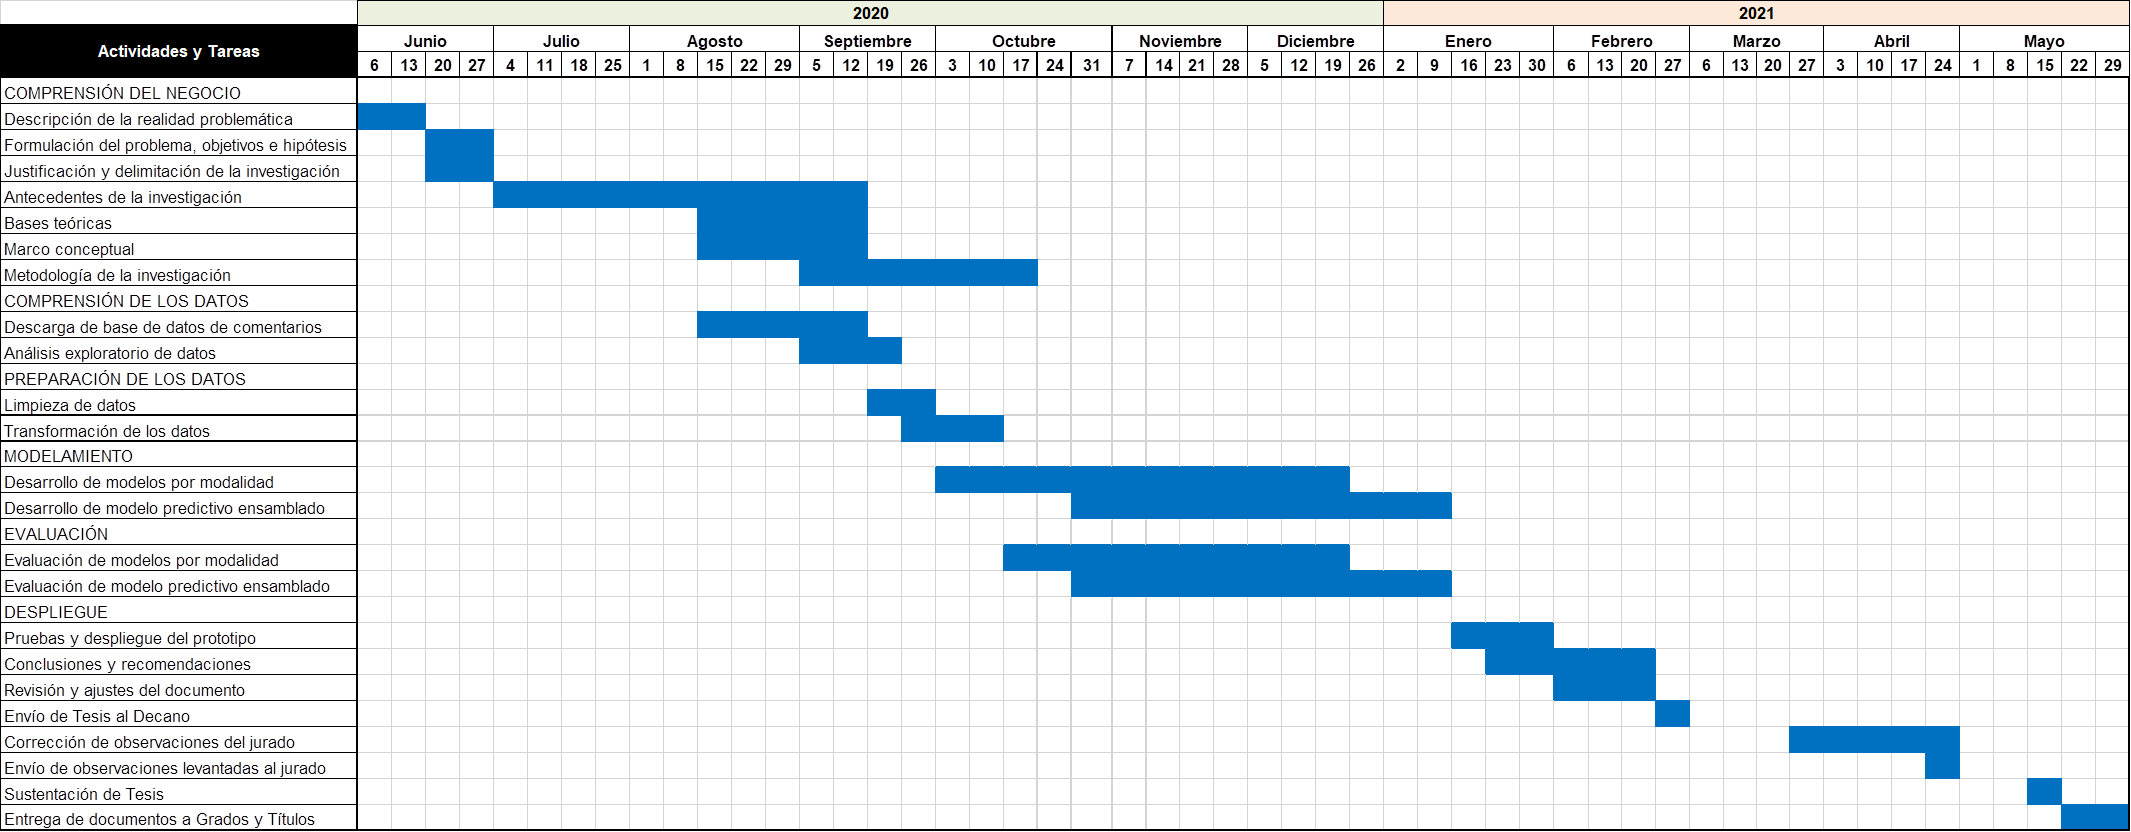
\includegraphics[width=1\textwidth]{3/figures/cronograma.png}
        \caption[Cronograma de actividades de la investigación]{Cronograma de actividades de la investigación, estructurado según las fases de la metodología CRISP-DM y distribuido a lo largo de los meses del período de ejecución.\
Fuente: Elaboración propia.}
        \label{4:fig7}
    \end{center}
\end{figure}
\end{landscape}
 
Los gastos asumidos por los autores para el desarrollo de la investigación se detallan en la Tabla \ref{4:table9}.

\begin{table}[h!]
\renewcommand\arraystretch{1.2}
\caption[Presupuesto de costos personales del autor]{Detalle del presupuesto correspondiente a los costos personales del autor en el desarrollo de la investigación.}
\label{4:table9}
\centering
\small
\begin{tabular}{lcrr}
\specialrule{.1em}{.05em}{.05em}
\multicolumn{1}{c}{\textbf{Ítem}} & \multicolumn{1}{c}{\textbf{Tiempo (horas)}} & \multicolumn{1}{c}{\textbf{Costo (soles)}} & \multicolumn{1}{c}{\textbf{Subtotal}} \\
\specialrule{.1em}{.05em}{.05em}
\multicolumn{4}{l}{\textbf{Recursos materiales}} \\
Equipo de cómputo para desarrollo (GPU integrada) & & S/.4,800.00 & S/.4,800.00 \\
\hline
\multicolumn{4}{l}{\textbf{Gestiones académicas}} \\
Matrícula en cursos de actualización y TSP & & S/.8,500.00 & S/.8,500.00 \\
\hline
\multicolumn{4}{l}{\textbf{Recursos humanos}} \\
Desarrollo del avance de tesis & 900 & No cuantificable & -- \\
\hline
\multicolumn{4}{l}{\textbf{Servicios generales}} \\
Internet y electricidad (5 meses) & 120 & S/.85.00 & S/.680.00 \\
\specialrule{.1em}{.05em}{.05em}
\textbf{Total} & & & \textbf{S/.14,880.00} \\
\specialrule{.1em}{.05em}{.05em}
\end{tabular}
\begin{flushleft}
\small Fuente: Elaboración propia.
\end{flushleft}
\end{table}
 
Los gastos asociados al uso de servicios en la nube, necesarios para el procesamiento del corpus y el entrenamiento de los modelos, se detallan en la Tabla \ref{4:table10}.

\begin{table}[h!]
\renewcommand\arraystretch{1.2}
\caption[Presupuesto de herramientas y servicios utilizados]{Detalle del presupuesto correspondiente a herramientas y servicios utilizados durante el desarrollo del sistema.}
\label{4:table10}
\centering
\small
\begin{tabular}{p{5.5cm} >{\centering\arraybackslash}p{4.5cm} p{5cm}}
\specialrule{.1em}{.05em}{.05em}
\multicolumn{1}{c}{\textbf{Ítem}} & \multicolumn{1}{c}{\textbf{Costo estimado}} & \multicolumn{1}{c}{\textbf{Notas}} \\
\specialrule{.1em}{.05em}{.05em}
\multicolumn{3}{l}{\textbf{Servicios y APIs en la nube}} \\
DeepSeek API (etiquetado LLM, $\sim$10k docs/mes) & $\sim$\$8 USD/mes & \$0.0008/doc con 85.5\% cache hit \\
\hline
TwitterAPI.io (acceso datos Twitter/X) & Variable & Alternativa a API oficial X \\
\hline
\multicolumn{3}{l}{\textbf{Infraestructura y bases de datos locales}} \\
Infraestructura de cómputo & \$0 & Docker sobre laptop/servidor propio \\
\hline
Neo4j Community Edition & \$0 & Sin cargo (reemplaza AuraDB) \\
\hline
PostgreSQL + pgvector & \$0 & Contenedor Docker local \\
\hline
\multicolumn{3}{l}{\textbf{Herramientas de extracción}} \\
YouTube / TikTok scraping & \$0 & \texttt{yt-dlp}, sin API de pago \\
\specialrule{.1em}{.05em}{.05em}
\textbf{Total aproximado} & \textbf{$\sim$\$8 USD/mes + costos variables} & \textbf{Dependiente del volumen de datos} \\
\specialrule{.1em}{.05em}{.05em}
\end{tabular}
\begin{flushleft}
\small Fuente: Elaboración propia.
\end{flushleft}
\end{table}